\documentclass[10pt,twocolumn]{article}
\usepackage[utf8]{inputenc}
\usepackage[T1]{fontenc}
\usepackage[english]{babel}
\usepackage{amsmath,amssymb}
\usepackage{geometry}
\geometry{a4paper, top=2.5cm, bottom=2.5cm, left=2cm, right=2cm, columnsep=0.6cm}
\usepackage{graphicx}
\usepackage{booktabs}
\usepackage{xcolor}
\usepackage{caption}
\captionsetup{font=small, labelfont=bf}
\renewcommand{\figurename}{Figur}
\renewcommand{\tablename}{Tabell}
\usepackage{natbib}
\bibliographystyle{apalike}
\usepackage[hidelinks]{hyperref}
\usepackage{titlesec}
\usepackage{fancyhdr}
\usepackage{lastpage}
\usepackage[most]{tcolorbox}
\newtcolorbox{omhugboks}{
  enhanced, colback=white, boxrule=0pt,
  borderline={0.4pt}{0pt}{black!55, dashed},
  left=5pt, right=5pt, top=3pt, bottom=3pt, arc=0pt,
  width=\columnwidth
}

% Colors
\definecolor{cMod}{RGB}{33,113,181}
\definecolor{cPal}{RGB}{35,139,69}
\definecolor{cVdL}{RGB}{203,24,29}
\definecolor{cKen}{RGB}{106,81,163}
\definecolor{gbg}{RGB}{235,235,235}

% Headers and footers (matching Eleganse style)
\pagestyle{fancy}
\fancyhf{}
\fancyhead[L]{\small\thepage}
\fancyhead[R]{\small\scshape\nouppercase{\rightmark}}
\renewcommand{\headrulewidth}{0.4pt}
\fancyfoot[R]{\small Page \thepage\ / \pageref{LastPage}}
\fancypagestyle{plain}{\fancyhf{}\fancyhead[L]{\small\thepage}\fancyhead[R]{\small\scshape Innleiing}\renewcommand{\headrulewidth}{0.4pt}\fancyfoot[R]{\small Page \thepage\ / \pageref{LastPage}}}

% Section formatting
\titleformat{\section}{\normalsize\bfseries}{\thesection}{0.6em}{}
\titleformat{\subsection}{\normalsize\bfseries\itshape}{\thesubsection}{0.5em}{}
\titlespacing*{\section}{0pt}{1.5ex plus 0.3ex minus 0.2ex}{0.6ex plus 0.1ex}
\titlespacing*{\subsection}{0pt}{1.0ex plus 0.2ex minus 0.1ex}{0.4ex plus 0.1ex}
\setlength{\parskip}{0pt}
\setlength{\parindent}{1em}
\setlength{\abovecaptionskip}{3pt}
\setlength{\belowcaptionskip}{1pt}
\setlength{\textfloatsep}{6pt}
\setlength{\floatsep}{4pt}
\setlength{\dbltextfloatsep}{6pt}
\setlength{\dblfloatsep}{4pt}
\setlength{\intextsep}{4pt}

\begin{document}

% ============================================================
% TITLE BLOCK (matching Eleganse style — single column)
% ============================================================
\twocolumn[%
\begin{flushleft}
{\LARGE\bfseries Proporsjonsgrammatikk og formgjevarkompetanse\par}
\vskip 0.3em
{\normalsize Ei komparativ analyse av fire historiske system gjennom Forml\ae re\par}
\vskip 0.6em
{\normalsize\bfseries Iver Raknes Finne}\quad{\small\texttt{iver.raknes.finne@stud.aho.no}}\quad{\small AHO\par}
\vskip 0.15em
{\small$\cdot$\quad 2026\par}
\end{flushleft}
\vskip 0.8em

% ============================================================
% SAMMANDRAG BOX (gray background, matching Eleganse style)
% ============================================================
\noindent\colorbox{gbg}{\parbox{0.97\textwidth}{\small\vspace{4pt}
\textbf{Sammandrag.}\quad Reduksjonsteoremet \citep[prop.~5.72]{Finne2026} formaliserer shape grammar \citep{StinyGips1972} og CK-teori \citep{HatchuelWeil2009} som degenererte grensetilfelle av Forml\ae re. Artikkelen instansierer teoremet p\aa{} fire historiske proporsjonsgrammatikkar: Le Corbusier sin Modulor (1948), den palladianske grammatikken \citep{StinyMitchell1978}, Van der Laan sitt plastiske tal ($\sim$1960), og ken/tatami-grammatikken ($\sim$10.\ hundre\aa ret). For Palladio er $|K|/|L(\mathbf{SG})| \leq 0{,}043$ \citep{StinyMitchell1978b}: over 95~\% av det grammatiske spr\aa ket ligg i $C \setminus K$. For dei tre andre systema gjev ingen tidlegare SG- eller CK-formalisering ei samanliknbar avstanding. Meta-teoremet \citep[prop.~7.15]{Finne2026} predikerer at sviktsignaturen klyngjer seg p\aa{} formgjevarens blindflekkar. Alle fire system stadfestar prediksjonen; det ledige h\o{}gplat\aa et i $C \setminus K$ kor h\o{}g grammatisk eleganse m\o{}ter h\o{}g industriell integrasjon forblir historisk urealisert.
\textbf{N\o{}kkelord:} Forml\ae re; shape grammar; CK-teori; kognitiv lyskjegle; omhug; Modulor; Van der Laan; Palladio; tatami\vspace{4pt}
}}
]

\section{Innleiing}

Formgrammatikken \citep{StinyGips1972,StinyMitchell1978,Benros2012,Duarte2005} og CK-teorien \citep{HatchuelWeil2009,Kazakci2009} er dei to mest formelt strenge rammeverka i designteori. Begge har uavhengig utvikla seg i fire tiår utan \aa{} m\o{}ta kvarandre; ingen av dei kan svare p\aa{} eit enkelt sp\o{}rsm\aa l: \emph{kvifor} er eit proporsjonssystem betre eigna langs visse aksar og svakare langs andre?

Forml\ae re \citep{Finne2026} svarar ved \aa{} innehalda begge som delstrukturar: shape grammar og CK-teori er degenererte grensetilfelle av kjerne-likninga \citep[prop.~5.72]{Finne2026}. Den fulle likninga er
\begin{equation}
\mathrm{Form} = \mathbf{SG}\bigl(\nabla_{C(A)} \mathcal{L}(c,t)\bigr),
\label{eq:core}
\end{equation}
der $\mathbf{SG}$ er formgrammatikken, $\mathcal{L}(c,t)$ tilpassingslandskapet for klasse $c$ ved tid $t$, og $\nabla_{C(A)}\mathcal{L}$ gradienten projisert p\aa{} agenten $A$ sin kognitive lyskjegle $C(A)$ \citep{FieldsLevin2022}. Denne artikkelen instansierer kjerne-likninga p\aa{} fire historiske proporsjonssystem og viser at sviktsignaturen til kvart system er predikerbar fr\aa{} formgjevaren si lyskjegle \citep[prop.~7.15]{Finne2026}.

\section{Teoretisk rammeverk}

\subsection{Forml\ae res designrom}
Designrommet til ein klasse er ein femdobbel $\mathbf{D} = (M, \Pi, \mathbf{SG}, \mathcal{L}, A)$:

\noindent
$M$ = formrommet (alle moglege konfigurasjonar)\\
$\Pi = (K, C, F)$ = epistemisk partisjon: busett, open, forboden\\
$\mathbf{SG} = (S, R, \omega)$ = formgrammatikk\\
$\mathcal{L}\colon M \to \mathbb{R}$ = tilpassingslandskap\\
$A = \{A_0, \ldots, A_n\}$ = fleirskalart agenthierarki

\subsection{Omhug og sviktsignatur}
Omhug er mengda av aksar agenten aktivt representerer \citep{FieldsLevin2022}. Proposisjon~7 sl\aa r fast at den realiserte forma er eit leseleg arkiv over kompromissets dimensjonalitet: svikten klyngjer seg n\o{}yaktig p\aa{} dei urepresenterte aksane. P\aa standen er falsifiserbar.

\subsection{Reduksjon og meta-teorem}
Reduksjonsteoremet \citep[prop.~5.72]{Finne2026} formulerer eksplisitt kva likning~\eqref{eq:core} reduserer til i grensetilfella: (i) rein formgrammatikk n\aa r $\nabla \mathcal{L} \equiv 0$, $|A| = 1$ og $\Pi = (M, \emptyset, \emptyset)$, som gjev $\mathrm{Form} = \mathbf{SG}(0) = L(\mathbf{SG})$; (ii) rein CK-teori n\aa r $\mathbf{SG} = \mathrm{id}_M$ og $\mathcal{L} = \mathbf{1}_K$, der operasjonane reduserer til partisjonsendringar mellom $K$ og $C$. Kvart grensetilfelle fjernar eitt lag av likninga. Meta-teoremet \citep[prop.~7.15]{Finne2026} gjev konsekvensen: rein SG genererer det moglege spr\aa ket men skil ikkje kva i spr\aa ket som vil svikte langs kva akse; rein CK partisjonerer $K$ og $C$ men utleier ikkje sviktsignatur. Prediksjon krev alle tre lag.

\section{Formrommet og dets aksar}

Tabell~\ref{tab:axes} kartlegg dei prim\ae re aksane i $M$. Desse aksane dannar grunnlaget for analysen og for tilpassingslandskapet i Figur~\ref{fig:landscape}.

\begin{table}[t]
\centering
\caption{Prim\ae re aksar i formrommet for proporsjonsreidskap. Var.: H = h\o{}g, M = moderat, L = l\aa g.}
\label{tab:axes}
\small
\begin{tabular}{@{}lr@{}}
\toprule
\textbf{Akse} & \textbf{Var.} \\
\midrule
Mat.\ grunnlag (irrasjonelt/heiltal/materielt) & H \\
Grammatisk eleganse / minimalisme & H \\
Intern logisk koherens & M \\
Kommuniserbarheit / pedagogisk klarheit & H \\
Industriell integrasjonsdjupn & H \\
Antropometrisk inklusjon (populasjonsvariasjon) & H \\
3D-spatial koherens (plan, rom, fasade) & H \\
Skaladekning (detalj til bystruktur) & M \\
Dynamisk ergonomi (rom i r\o{}rsle) & L \\
\bottomrule
\end{tabular}
\end{table}

\section{Analyse av dei fire systema}

\subsection{Modulor (Le Corbusier, 1948)}

\textbf{SG-laget.} Modulor er skalainvariant og bimodal: to interleava geometriske seriar p\aa{} gylne snitt $\varphi = (1+\sqrt{5})/2 \approx 1{,}618$,
\begin{equation}
r_{n+1} = \varphi\, r_n, \qquad b_n = \varphi\, r_n,
\end{equation}
forankra p\aa{} referanseh\o{}gd 1,83~m. \citet{Watanabe2020} enumerte panel-kombinasjonane algoritmisk og stadfesta at talrommet er kombinatorisk rikt. \textbf{CK-laget.} $K$ = Unit\'e-typologien; $C \setminus K$ inneheld $\varphi$-konfigurasjonar i industriell produksjon som Le Corbusier sj\o{}lv aldri fors\o{}kte \aa{} l\o{}ysa. \textbf{Kompetanse-laget:}

\begin{figure}[t]
\centering
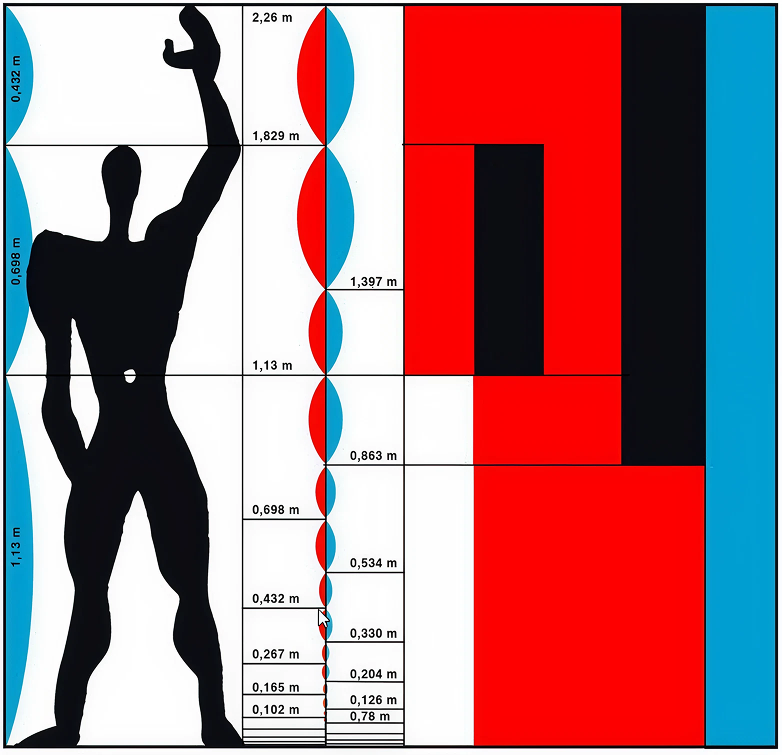
\includegraphics[width=0.7\columnwidth]{../figures/formgjevarkompetanse/figur_1-le-corbusier.png}
\caption{Modulor: bimodal proporsjonserie (raud og bl\aa{} serie) p\aa{} gylne snitt, referansekropp 1,83~m.}
\label{fig:modulor}
\end{figure}

\begin{omhugboks}
\small\textbf{H\o{}g omhug:} proporsjonell harmoni $\cdot$ kommuniserbarheit $\cdot$ skaladekning $\cdot$ pedagogisk klarheit\\[1pt]
\textbf{Blindflekkar:} industriell integrasjon $\cdot$ befolkningsvariasjon $\cdot$ dynamisk ergonomi
\end{omhugboks}

Referanseh\o{}gda 1,83~m samsvara ikkje med gjennomsnittsh\o{}gda i den franske befolkninga (1,60--1,69~m) \citep{LorenzoPalomera2022}; kvinner og born er eksplisitt ekskluderte \citep{Buzzi2017}. $\varphi$-baserte m\aa l harmonerer ikkje med standardmurverk. Svikten fell der prop.~7.15 predikerer han.

\subsection{Den palladianske grammatikken (Palladio $\sim$1570)}

\textbf{SG-laget.} \citet{StinyMitchell1978} formaliserte villaplanane som ein parametrisk grammatikk med ni reglar i \'atte stadium (Figur~\ref{fig:palladio}); \citet{Duarte2005} og \citet{Benros2012} har sidan utvida formaliseringa. Reglane operer p\aa{} planform, romform og fasadeform \emph{simultant}, og bevarer heiltalstilh\o{}va 1:1, 2:3, 3:4, 4:6 \citep{Wittkower1949,MarchStiny1985} p\aa{} tvers av alle tre. \textbf{CK-laget.} $K = 10$ realiserte villaer; grammatikken genererer $|L(\mathbf{SG})| \geq 230$ plan \citep{StinyMitchell1978b}. Forholdstalet $|K|/|L(\mathbf{SG})| \leq 0{,}043$ gjer CK-asymmetrien kvantitativ: over 95~\% av det grammatiske spr\aa ket ligg i $C \setminus K$. \textbf{Kompetanse-laget:}

\begin{omhugboks}
\small\textbf{H\o{}g omhug:} 3D-spatial koherens $\cdot$ proporsjonell harmoni $\cdot$ matematisk eleganse $\cdot$ skaladekning\\[1pt]
\textbf{Blindflekkar:} konstruksjonsmaterial $\cdot$ antropometri $\cdot$ urban kontekst
\end{omhugboks}

\begin{figure}[t]
\centering
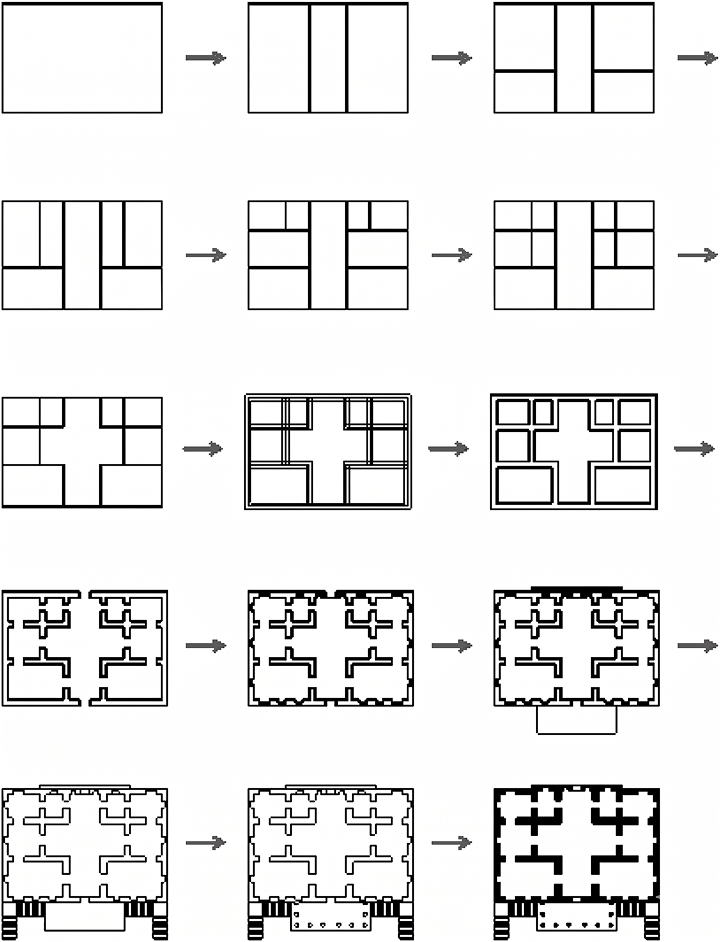
\includegraphics[width=\columnwidth]{../figures/formgjevarkompetanse/figur_2b-palladio-derivasjon.png}
\caption{Palladiansk grammatikk: stegvis derivasjon fr\aa{} grunnform til ferdig villaplan \citep{StinyMitchell1978}.}
\label{fig:palladio}
\end{figure}

\subsection{Det plastiske talet (Van der Laan, $\sim$1960)}

\textbf{SG-laget.} Ein minimal grammatikk: konstant $\rho \approx 1{,}3247$ definert av $\rho^3 = \rho + 1$, og rekursjonsregelen $x_{n+3} = x_n + x_{n+1}$ (Padovan-sekvensen: $1, 1, 1, 2, 2, 3, 4, 5, 7, 9, 12, 16, 21, 28, \ldots$). Tre suksessive potensar $1:\rho:\rho^2$ gjev breidd, h\o{}gd og djupn som eit nativt 3D-tilh\o{}ve (Figur~\ref{fig:vdl}) \citep{VanderLaan1977,Padovan1994,Padovan2002,ProiettiDenBiesen2025}. Der $\varphi$ er \'eindimensjonalt, er $\rho$ tredimensjonalt. Ingen publisert SG- eller CK-formalisering eksisterer for systemet. \textbf{CK-laget.} $|K| \approx 1$: Abdij van Vaals og ein tynn monastisk linje. $|C \setminus K|$ er enormt. \textbf{Kompetanse-laget:}

\begin{omhugboks}
\small\textbf{H\o{}g omhug:} matematisk minimalisme $\cdot$ 3D-spatial koherens $\cdot$ proporsjonell harmoni\\[1pt]
\textbf{Blindflekkar:} kommuniserbarheit $\approx 0$ $\cdot$ industriell integrasjon $\approx 0$
\end{omhugboks}

\begin{figure}[t]
\centering
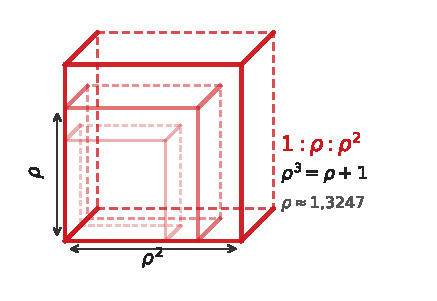
\includegraphics[width=0.85\columnwidth]{../figures/formgjevarkompetanse/fig_vanderlaan.pdf}
\caption{Van der Laan: nesta volum $1:\rho:\rho^2$ der $\rho^3=\rho+1$ \citep{Padovan2002}.}
\label{fig:vdl}
\end{figure}

\subsection{Ken/tatami-grammatikken (Japan, $\sim$10.\ hundre\aa ret)}

\textbf{SG-laget.} \citet{Knight1981} gav ein parametrisk grammatikk med 41 reglar for japansk te-rom p\aa{} ken/tatami-gridet (Figur~\ref{fig:tatami}): ein tatami-matte er $\tfrac{1}{2}\,\text{ken} \times 1\,\text{ken}$ ($\approx 0{,}91 \times 1{,}82$~m), tilh\o{}vet 1:2 er invariant, og rom har storleik $N$ tatami for $N \in \{2, 3, 4{,}5, 6, 8, 10\}$. \textbf{CK-laget.} $K$ dekkjer eit stort historisk korpus; det radikale er at grammatikk-eininga \emph{er} konstruksjonseininga---ei kollapsa skilje som avgrensar $C$. \textbf{Kompetanse-laget.} Formgjevaren er ein kumulativ, anonym, multi-skalar agent over fleire hundre \aa r---empirisk realisasjon av Forml\ae res $A = \{A_0, \ldots, A_n\}$.

\begin{omhugboks}
\small\textbf{H\o{}g omhug:} industriell integrasjon $\cdot$ kommuniserbarheit $\cdot$ antropometrisk inklusjon $\cdot$ intern koherens\\[1pt]
\textbf{Blindflekkar:} estetisk generativitet $\cdot$ universell overf\o{}ring
\end{omhugboks}

\begin{figure}[t]
\centering
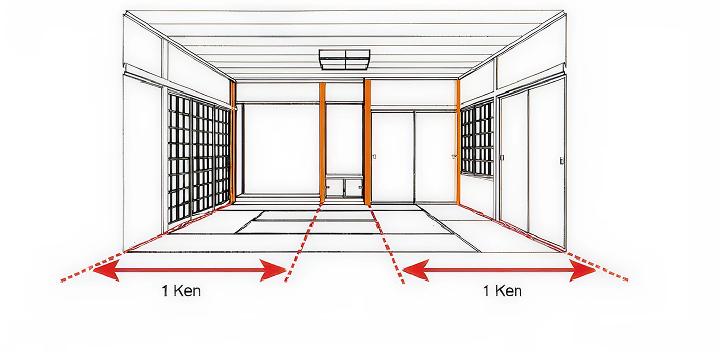
\includegraphics[width=\columnwidth]{../figures/formgjevarkompetanse/figur_4a-ken-modul-perspektiv.png}
\caption{Ken/tatami: grammatikk-eining og konstruksjonseining er den same fysiske gjenstanden. Tilh\o{}vet 1:2 er invariant \citep{Engel1985}.}
\label{fig:tatami}
\end{figure}

\section{Komparativ diagnose}

\subsection{Kognitiv lyskjegle og sviktsignatur}
Figur~\ref{fig:lightcone} viser kompetanse-laget eksplisitt: kvar formgjevar si lyskjegle (dei aksane som er aktivt representerte), og kvar sviktsignaturen forventast. M\o{}rke armar er innanfor lyskjegla; bleike armar er delvis; stipla armar med kryss er blindflekkar. Meta-teoremet predikerer at svikt klyngjer seg p\aa{} krysspunkta.

\begin{figure}[t]
\centering
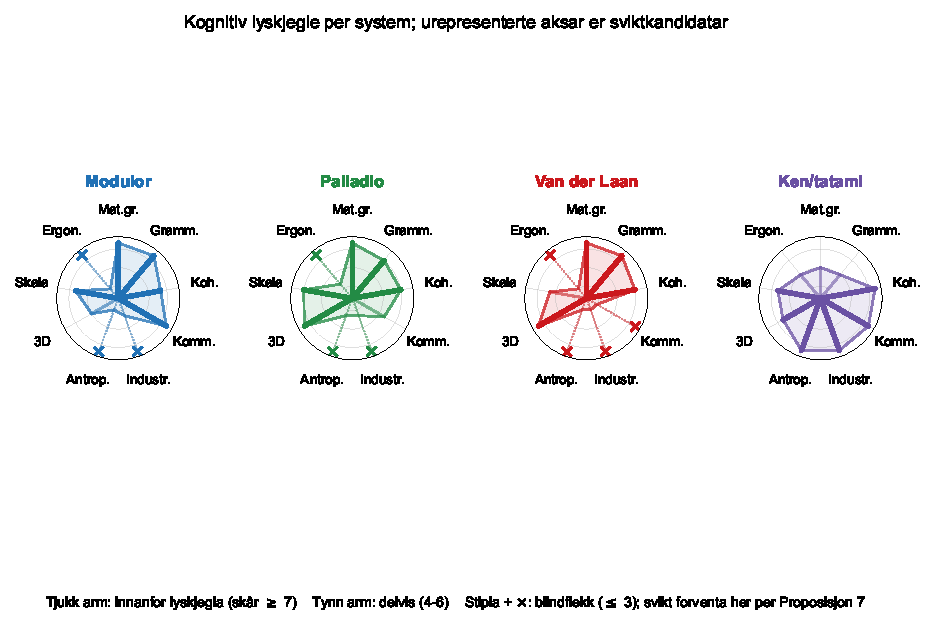
\includegraphics[width=\columnwidth]{../figures/formgjevarkompetanse/fig2_lightcone.pdf}
\caption{Kognitiv lyskjegle per system. Tjukke armar: innanfor lyskjegla ($\geq 7$). Tynne: delvis (4--6). Stipla + kryss: blindflekk ($\leq 3$), der svikt er forventa.}
\label{fig:lightcone}
\end{figure}

Asymmetrien er analytisk produktiv: Modulor dominerer pedagogisk kommunikasjon og formgrammatisk eleganse; Palladio trimodal spatial koherens; Van der Laan matematisk minimalisme i nativ 3D; Ken/tatami grammatikk-material-kollaps der integrasjonsproblemet er ein logisk umogleg kategori---ikkje ei utfordring \aa{} l\o{}ysa.

\subsection{Tilpassingslandskapet og det ledige h\o{}gplat\aa et}
Figur~\ref{fig:landscape} viser CK-laget eksplisitt: dei fire systema som lokale maksima i $K$, og eit ledig h\o{}gplat\aa{} i $C \setminus K$ der h\o{}g grammatisk eleganse m\o{}ter h\o{}g industriell integrasjon. Konfigurasjonen er tenkeleg, ikkje n\o{}dvendigvis forbode, og ingen av dei fire okkuperer han. Tilpassingslandskapet er genuint fleirtoppa.

\begin{figure}[t]
\centering
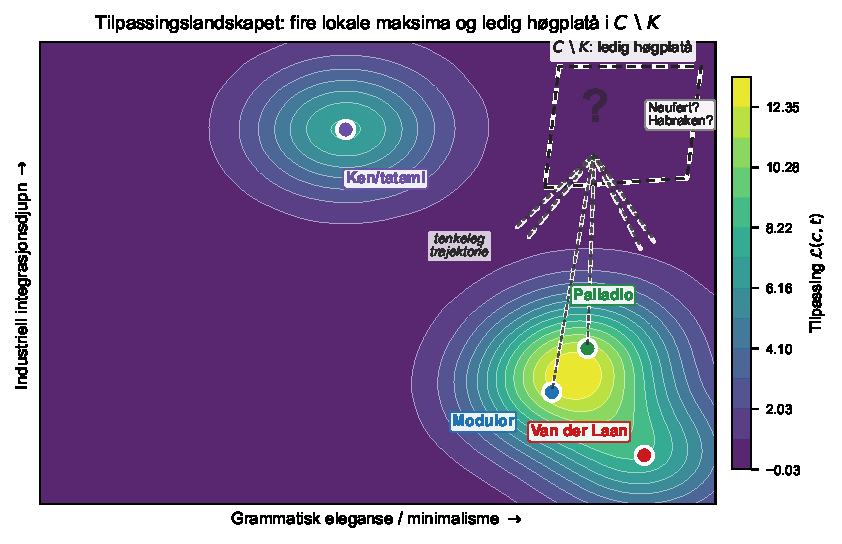
\includegraphics[width=\columnwidth]{../figures/formgjevarkompetanse/fig3_landscape.pdf}
\caption{Tilpassingslandskapet $\mathcal{L}(c,t)$ p\aa{} grammatisk eleganse ($x$) og industriell integrasjonsdjupn ($y$). Stipla omriss: ledig h\o{}gplat\aa{} i $C \setminus K$.}
\label{fig:landscape}
\end{figure}

\subsection{CK-operatorane Forml\ae re aktiverer}
Diagnosen svarar til CK-operatorane (Figur~\ref{fig:cksquare}): \emph{asymmetrisk diagnose} er $K \rightarrow K$, \emph{sviktprediksjon} er $K \rightarrow C$, og \emph{h\o{}gplat\aa-identifikasjon} er $C \rightarrow K$.

\begin{figure}[t]
\centering
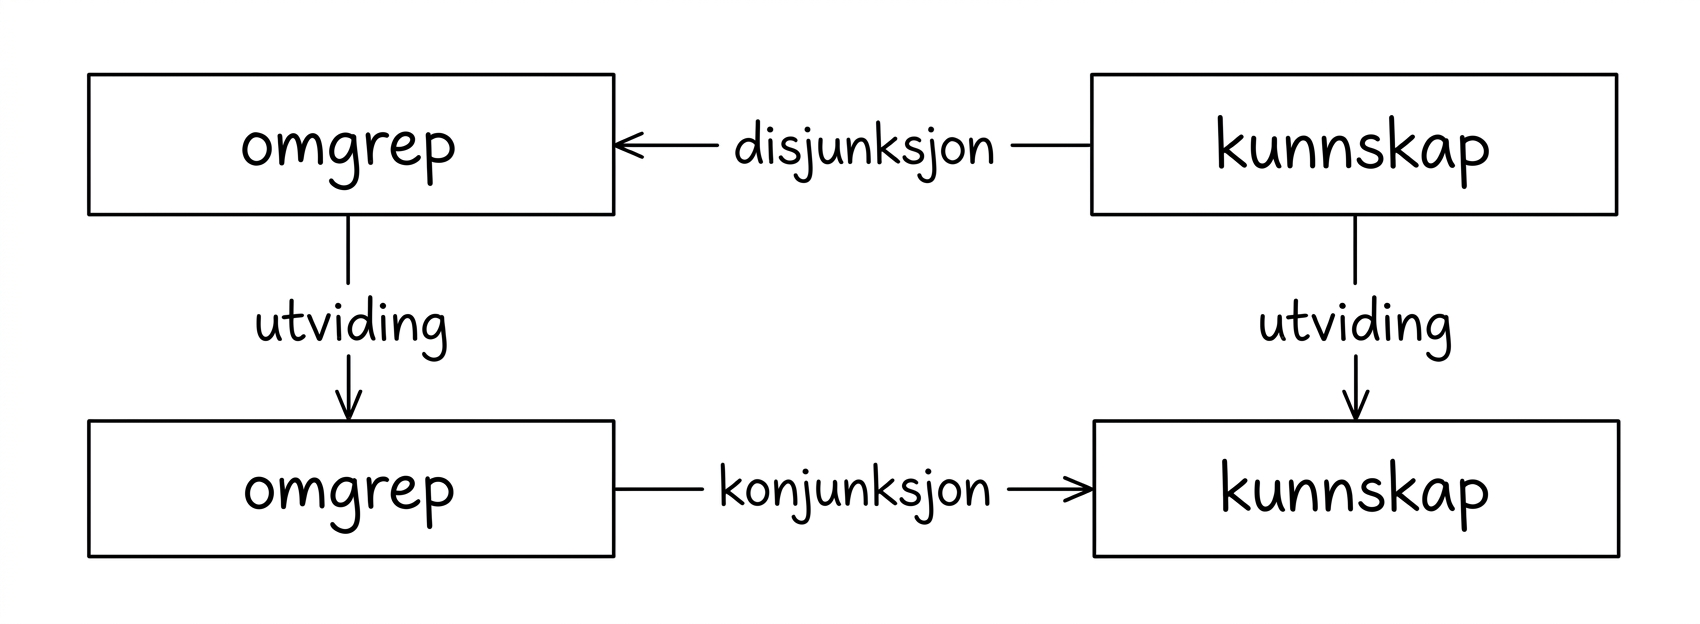
\includegraphics[width=0.9\columnwidth]{../figures/formgjevarkompetanse/figur_4-ck-design-square.png}
\caption{CK-kvadratet \citep{HatchuelWeil2009}. Forml\ae re opererer p\aa{} alle fire operatorane: $K\rightarrow K$ (samanlikning), $K\rightarrow C$ (sviktprediksjon), $C\rightarrow K$ (h\o{}gplat\aa-identifikasjon).}
\label{fig:cksquare}
\end{figure}

\subsection{Klassebasert evaluering}
Skiljet mellom kva systemet \emph{er} eit reidskap for og kva det \emph{har vorte brukt som} er operasjonelt: den antropometriske kritikken av Modulor \citep{LorenzoPalomera2022} er korrekt og viktig, men stiller eit sp\o{}rsm\aa l Modulor aldri eksplisitt lova \aa{} svara. Forml\ae re lokaliserer kritikken som ein $K\rightarrow C$-ekstensjon: han namngjev ein tenkeleg utvida Modulor, ikkje ein svikt i den historiske.

\section{Diskusjon}

\subsection{Prediktiv case: Neufert p\aa{} h\o{}gplat\aa et}
Neufert sin \emph{Bauentwurfslehre} (1936--) kvalifiserer som kandidat i $C \setminus K$: h\o{}g industriell integrasjonsdjupn, moderat grammatisk eleganse, men antropometrisk skeivheit parallell til Modulor (mannleg referansekropp; tunn dekning av variasjon). Per meta-teoremet \citep[prop.~7.15]{Finne2026} predikerer Forml\ae re at sviktsignaturen klyngjer seg p\aa{} dynamisk ergonomi og ikkje-standard-kroppar---testbart mot den faktiske Neufert-kritikken. Operatoren er $C \rightarrow K$: ei tidlegare tenkeleg konfigurasjon reintegrert som eit f\o{}rehandsbildet kompetanseprofil.

\subsection{N=4 og falsifikasjonsrommet}
Fire post hoc-saker er demonstrasjon, ikkje statistisk test. Falsifikasjon krev eit system der kartlagd blindflekk og historisk sviktsignatur \emph{divergerer}; ingen av dei fire gjer det. Konsistens er ikkje generalitet. Neufert-prediksjonen er f\o{}rste steg mot prospektiv testing.


\section{Konklusjon}

Formrommet for proporsjonsreidskap er fleirtoppa. Kvar formgjevar si lyskjegle gjev ein unik omhugssignatur og ein predikerbar sviktsignatur. Ingen av dei fire systema dominerer globalt; det ledige h\o{}gplat\aa et forblir i $C \setminus K$. Det epistemologisk avgjerande bidraget er at Forml\ae re, fordi ho inneheld SG og CK som delstrukturar, gjer skiljet mellom kva eit system \emph{er} og kva det \emph{vert brukt som} operasjonelt og falsifiserbart.

\subsection*{Forfattarerkl\ae ring}
Ingen interessekonfliktar. Ingen ekstern finansiering.

\begin{thebibliography}{99}
\footnotesize
\setlength{\itemsep}{0pt}
\setlength{\parskip}{0pt}

\bibitem[Benros et al., 2012]{Benros2012}
Benros, D., Hanna, S., \& Duarte, J. P. (2012). A new Palladian shape grammar: A subdivision grammar as alternative. \emph{International Journal of Architectural Computing}, \emph{10}(4), 521--540. \url{https://doi.org/10.1260/1478-0771.10.4.521}

\bibitem[Buzzi, 2017]{Buzzi2017}
Buzzi, F. (2017). `Human, all too human': A critique on the Modulor. \emph{Failed Architecture}. \url{https://failedarchitecture.com/human-all-too-human-a-critique-on-the-modulor/}

\bibitem[Cohen, 2014]{Cohen2014}
Cohen, J.-L. (2014). Le Corbusier's Modulor and the debate on proportion in France. \emph{Architectural Histories}, \emph{2}(1), 1--16. \url{https://doi.org/10.5334/ah.bv}

\bibitem[Duarte, 2005]{Duarte2005}
Duarte, J. P. (2005). A Palladian construction grammar: Design reasoning with shape grammars and rapid prototyping. \emph{Environment and Planning B: Planning and Design}, \emph{32}(3), 347--380. \url{https://doi.org/10.1068/b31147}

\bibitem[Engel, 1985]{Engel1985}
Engel, H. (1985). \emph{Measure and construction of the Japanese house}. Tuttle.

\bibitem[Fields \& Levin, 2022]{FieldsLevin2022}
Fields, C., \& Levin, M. (2022). Competency in navigating arbitrary spaces as an invariant for analyzing cognition in diverse embodiments. \emph{Entropy}, \emph{24}(6), 819. \url{https://doi.org/10.3390/e24060819}

\bibitem[Finne, 2026]{Finne2026}
Finne, I. R. (2026). \emph{Forml\ae re: Ein formell teori om designkompetanse, formrom og seleksjonstrykk} [Upublisert manuskript]. Arkitektur- og designh\o{}gskolen i Oslo.

\bibitem[Hatchuel \& Weil, 2009]{HatchuelWeil2009}
Hatchuel, A., \& Weil, B. (2009). C-K design theory: An advanced formulation. \emph{Research in Engineering Design}, \emph{19}(4), 181--192. \url{https://doi.org/10.1007/s00163-008-0043-4}

\bibitem[Kazakci, 2009]{Kazakci2009}
Kazakci, A. O. (2009). \emph{Imagining knowledge: A formal account of design as a C-K process} [Working paper]. HAL. \url{https://minesparis-psl.hal.science/hal-00983061}

\bibitem[Knight, 1981]{Knight1981}
Knight, T. W. (1981). The forty-one steps. \emph{Environment and Planning B: Planning and Design}, \emph{8}(1), 97--114. \url{https://doi.org/10.1068/b080097}

\bibitem[Krishnamurti et al., 2011]{Krishnamurti2011}
Krishnamurti, R., Tsamir, P., \& Rinaldi, M. (2011). Modularity and proportions in architecture and their relevance to a generative approach to architectural design. \emph{Nexus Network Journal}, \emph{13}(2), 297--312. \url{https://doi.org/10.1007/s00004-011-0097-x}

\bibitem[Lorenzo-Palomera et al., 2022]{LorenzoPalomera2022}
Lorenzo-Palomera, J., Fuentes-P\'erez, C., \& Aranda-Jim\'enez, Y. (2022). Le Corbusier's Modulor: Anthropometric myth. \emph{Civil Engineering and Architecture}, \emph{10}(1), 112--120. \url{https://doi.org/10.13189/cea.2022.100110}

\bibitem[March \& Stiny, 1985]{MarchStiny1985}
March, L., \& Stiny, G. (1985). Spatial systems in architecture and design: Some history and logic. \emph{Environment and Planning B: Planning and Design}, \emph{12}(1), 31--53. \url{https://doi.org/10.1068/b120031}

\bibitem[Padovan, 1994]{Padovan1994}
Padovan, R. (1994). \emph{Dom Hans van der Laan: Modern primitive}. Architectura \& Natura.

\bibitem[Padovan, 2002]{Padovan2002}
Padovan, R. (2002). Dom Hans van der Laan and the plastic number. \emph{Nexus Network Journal}, \emph{4}(3), 181--193. \url{http://www.emis.ams.org/journals/NNJ/conferences/N2002-Padovan.html}

\bibitem[Proietti \& den Biesen, 2025]{ProiettiDenBiesen2025}
Proietti, T., \& den Biesen, K. (2025). \emph{Hans van der Laan's instruments of thought: Proportion, architecture, analogy}. Routledge.

\bibitem[Rozhkovskaya, 2019]{Rozhkovskaya2019}
Rozhkovskaya, A. (2019). \emph{Mathematical commentary on Le Corbusier's Modulor}. Kansas State University. \url{https://math.ksu.edu/~rozhkovs/Modulor_oct19final.pdf}

\bibitem[Stiny \& Gips, 1972]{StinyGips1972}
Stiny, G., \& Gips, J. (1972). Shape grammars and the generative specification of painting and sculpture. \emph{Information Processing}, \emph{71}, 1460--1465.

\bibitem[Stiny \& Mitchell, 1978a]{StinyMitchell1978}
Stiny, G., \& Mitchell, W. J. (1978a). The Palladian grammar. \emph{Environment and Planning B: Planning and Design}, \emph{5}(1), 5--18. \url{https://doi.org/10.1068/b050005}

\bibitem[Stiny \& Mitchell, 1978b]{StinyMitchell1978b}
Stiny, G., \& Mitchell, W. J. (1978b). Counting Palladian plans. \emph{Environment and Planning B: Planning and Design}, \emph{5}(2), 189--198. \url{https://doi.org/10.1068/b050189}

\bibitem[Van der Laan, 1977]{VanderLaan1977}
Van der Laan, H. (1977). \emph{De architectonische ruimte}. Brill.

\bibitem[Watanabe, 2020]{Watanabe2020}
Watanabe, M. S. (2020). Exploring the panel exercises in the Modulor as presented by Le Corbusier. \emph{Japan Architectural Review}, \emph{3}(4), 442--453. \url{https://doi.org/10.1002/2475-8876.12147}

\bibitem[Wittkower, 1949]{Wittkower1949}
Wittkower, R. (1949). \emph{Architectural principles in the age of humanism}. Warburg Institute.

\end{thebibliography}

\end{document}
